\chapter{Fonctions polynôme de dégré 2}
\thispagestyle{fancy}

\section{Forme développée}

	\begin{spacing}{1.7}
    \begin{bdefi}
    	\ \\
        \pointille[\textwidth]
        \pointille[\textwidth]
        \pointille[\textwidth]
        \pointille[\textwidth]
    \end{bdefi}
	\end{spacing}
    
    \begin{brmq}
        Une fonction polynôme de degré 2 s'appelle également fonction trinôme du second degré ou par abus de langage \guillemets{trinôme}.
    \end{brmq}

	\begin{bmanip}
		Sur le logiciel GeoGebra  $\vcenter{\hbox{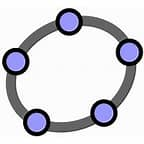
\includegraphics[height=1.2\baselineskip]{ggb-icon}}}$ créer trois curseurs $a, b, c$ puis dans la ligne de saisie taper $f(x)=a x^2+b x+c$. On obtient ainsi le tracé de la courbe représentative de la fonction $f$ définie par $f(x)=a x^2+b x+c$ on s'intéressera aux cas où $a \neq 0$. (si $a=0 f$ est une fonction affine)
	\end{bmanip}

	\begin{spacing}{1.7}
	\begin{bdefi}
		La courbe représentative d'une fonction polynôme du second degré est appelée \pointille[3cm].
	\end{bdefi}
	\end{spacing}
    
    \begin{bexemple}
        \begin{itemEx}
            \item $f(x)=2\mRouge{x^2}-5x+2$ ou $g(x)=(\mRouge{x}-4)(5-2\mRouge{x})$ sont des fonctions polynômes de degré 2.
            \item $h(x)=5\mRouge{x}-3$ est une fonction polynôme de degré 1.
            \item $i(x)=5\mRouge{x^4}-7x^3+3x-8$  est une fonction polynôme de degré 4.
            
        \end{itemEx}
    \end{bexemple}

	\subsection*{Variations de la fonction trinôme}
	
	\begin{bmanip}
		Sur le logiciel GeoGebra  $\vcenter{\hbox{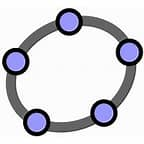
\includegraphics[height=1.2\baselineskip]{ggb-icon}}}$, reprendre la manipulation précédente et prendre un $a>0$. Faire alors varier $b$ et $c$. Que constatez-vous quant variations de $f$? Et si on prend un autre $a$ strictement positif? Conjecturer les variations de $f$ en complétant le tableau de variation suivant :\\
		1er cas $a>0$ :
		\begin{tikzpicture}
			\tkzTabInit{$x$ / 1 , $f(x)$ / 2}{\phantom{$-\infty$}, \phantom{$-\dfrac{b}{2a}$}, \phantom{$+\infty$}}
			\tkzTabVar{}
		\end{tikzpicture}
		
	\end{bmanip}

	\begin{bmanip}
		Sur le logiciel GeoGebra  $\vcenter{\hbox{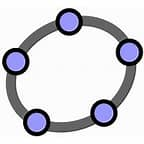
\includegraphics[height=1.2\baselineskip]{ggb-icon}}}$, reprendre la manipulation précédente et prendre un $a<0$. Faire alors varier $b$ et $c$. Que constatez-vous quant variations de $f$? Et si on prend un autre $a$ strictement négatif? Conjecturer les variations de $f$ en complétant le tableau de variation suivant :\\
		2ème cas $a<0$ :
		\begin{tikzpicture}
			\tkzTabInit{$x$ / 1 , $f(x)$ / 2}{\phantom{$-\infty$}, \phantom{$-\dfrac{b}{2a}$}, \phantom{$+\infty$}}
			\tkzTabVar{}
		\end{tikzpicture}
	\end{bmanip}
		Nous retiendrons donc : 
	\begin{bprop}
		\begin{minipage}[c]{0.5\linewidth}
			Si $a>0$
			\ \\
			
			\begin{tikzpicture}
				\tikzset{node style/.append style = {fill=none}}
				\tkzTabInit[lgt = 1.6, espcl = 2.4, deltacl = 0.5]{$x$ / 1 , $f(x)$ / 2}{$-\infty$, $x_S$, $+\infty$}
				\tkzTabVar{ }
			\end{tikzpicture}
		\end{minipage}
		\begin{minipage}[c]{0.5\linewidth}
			Si $a<0$
			\ \\
			
			\begin{tikzpicture}
				\tikzset{node style/.append style = {fill=none}}
				\tkzTabInit[lgt = 1.6, espcl = 2.4, deltacl = 0.5]{$x$ / 1 , $f(x)$ / 2}{$-\infty$, $x_S$, $+\infty$}
				\tkzTabVar{}
			\end{tikzpicture}
		\end{minipage}
	\end{bprop}

	\begin{bdefi}
		le point de coordonnés $\left(x_S ; y_S\right)$ avec $y_S$ l'extremum de $f$ sur $\mathrm{P}$ est appelé \grasInDef{sommet de la parabole}.
	\end{bdefi}
    
\section{Forme canonique d'une fonction polynôme de degré 2}
       
    \begin{spacing}{1.7}    
    \begin{bprop}
        Toute fonction polynôme f de degré 2 définie sur \R par $f(x)=ax^2+bx+c$ peut s'écrire sous la forme :\\
		\pointille[\textwidth]
		\pointille[\textwidth]
		\pointille[\textwidth]
		\pointille[\textwidth] 
    \end{bprop}
	\end{spacing}
    
    \begin{bdemo}
        Faite sur le cahier.
    \end{bdemo}

	\begin{bmanip}
		Sur le logiciel GeoGebra  $\vcenter{\hbox{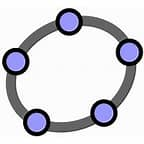
\includegraphics[height=1.2\baselineskip]{ggb-icon}}}$ créer trois curseurs $a, \alpha, \beta$ puis dans la ligne de saisie taper $f(x)=a(x-\alpha)^2+\beta$. On obtient ainsi le tracé de la courbe représentative de la fonction $f$ définie par $f(x)=a(x-\alpha)^2+\beta$. Compléter alors le cas général ci-dessous.
	\end{bmanip}

	\begin{bprop}
		\ \\
		Le sommet S a pour coordonnées \pointille[3cm]
	\end{bprop}

	\begin{spacing}{1.7}
	\begin{bprop}
		\ \\
		La parabole possède un \pointille[5cm]. Il s'agit de la droite d'équation \pointille[4cm].
	\end{bprop}
	\end{spacing}

	Avec ces nouvelles données, on peut maintenant compléter notre tableau de variations : 
	
	\begin{bprop}
		\begin{minipage}[c]{0.5\linewidth}
			Si $a>0$
			\ \\
			
			\begin{tikzpicture}
				\tikzset{node style/.append style = {fill=none}}
				\tkzTabInit[lgt = 1.6, espcl = 2.4, deltacl = 0.5]{$x$ / 1 , $f(x)$ / 2}{$-\infty$, \phantom{$\alpha$}, $+\infty$}
				\tkzTabVar{}
			\end{tikzpicture}
		\end{minipage}
		\begin{minipage}[c]{0.5\linewidth}
			Si $a<0$
			\ \\
			
			\begin{tikzpicture}
				\tikzset{node style/.append style = {fill=none}}
				\tkzTabInit[lgt = 1.6, espcl = 2.4, deltacl = 0.5]{$x$ / 1 , $f(x)$ / 2}{$-\infty$, \phantom{$\alpha$}, $+\infty$}
				\tkzTabVar{}
			\end{tikzpicture}
		\end{minipage}
	\end{bprop}

	\section{passage de la forme développée à la forme canonique}
	
	Pour passer de la forme développée à la forme canonique, il existe 2 méthodes
	
	\subsection{passer à la forme canonique à l'aide d'identité remarquable}
    
    
    
    \begin{bmethodet}{Déterminer la forme canonique d'une fonction polynôme de degré 2}
        \grasInMet{Enoncé :} 
        
        Soit la fonction f définie sur \R par : $f(x)=2x^2-20x+10$.
        
        On veut exprimer la fonction $f$ sous sa forme canonique.
        
        \grasInMet{Réponse :}
        
        \begin{spacing}{1.7}
        f doit être de la forme : 	
 		$f(x)=a(x-\alpha)^2+\beta$ 	
 		ou $a$, $\alpha$ et $\beta$ sont des nombres réels.
        
        On commence par mettre le $a$ en facteur pour les 2 termes avec des $x$
        
        \pointille[\textwidth]
          
        On fait ensuite apparaitre le 3ème terme d'une identité remarquable ($a^2\pm2ab+b^2$)
        
        \pointille[\textwidth]
        
        On factorise l'identité remarquable et on regroupe les termes qui restent ensemble.
        
        \pointille[\textwidth]
        
        \pointille[\textwidth]
        
        \pointille[\textwidth]

        \pointille[6cm] est la forme canonique de $f$.
    	\end{spacing}
    \end{bmethodet}


	\subsection{Cas général}
	
	\begin{spacing}{1.7}
	\begin{bprop}
		Pour passer de la forme développée à la forme canonique (ou inversement), on peut utiliser les formules:
		\pointille[5cm] et \pointille[5cm].\\
	\end{bprop}
	\end{spacing}

	\begin{bexemple}
		Soit la fonction f définie sur \R par : $f(x)=3x^2+60x-20$.
		On veut exprimer la fonction $f$ sous sa forme canonique.\\
		\ \\
		On commence par calculer $\alpha$:
		$\alpha=- \dfrac{b}{2a}=-\dfrac{60}{2\times 3}=-10$.
		\ \\
		Pour calculer $\beta$, on a 2 possibilités : soit on utilise la formule ci-dessus, soit on dit que $\beta=f(\alpha)$ et on remplace $x$ par $\alpha$ dans l'expression $f(x)$
	\end{bexemple}
    


